%File: formatting-instruction.tex
\documentclass[letterpaper]{article}
\usepackage{aaai}
\usepackage{times}
\usepackage{helvet}
\usepackage{courier}
\usepackage{amsmath,amssymb}
\usepackage[pdftex]{graphicx}
\usepackage[usenames]{color}

\newcommand{\Z}{\mathbb{Z}}
\newcommand{\R}{\mathbb{R}}
\newcommand{\cp}{CP Optimizer}

% Macro for colored "todo" notes:
\definecolor{NoteColor}{rgb}{1, 0.2, 0.2}
\newcommand{\note}[1]{\textcolor{NoteColor}{#1}}

% Macros for math functions:
\DeclareMathOperator{\dom}{dom}
\DeclareMathOperator{\exec}{exec}
\DeclareMathOperator{\EndBeforeStart}{endBeforeStart}   % the macro endBeforeStart is already defined, therefore the big E at the beginning
\DeclareMathOperator{\Span}{span}                       % same for the span
\DeclareMathOperator{\alternative}{alternative}
\DeclareMathOperator{\length}{length}
\DeclareMathOperator{\alwaysIn}{alwaysIn}
\DeclareMathOperator{\heightAtStart}{heightAtStart}
\DeclareMathOperator{\stepAtStart}{stepAtStart}
\DeclareMathOperator{\first}{first}
\DeclareMathOperator{\last}{last}
\DeclareMathOperator{\before}{before}
\DeclareMathOperator{\prev}{prev}
\DeclareMathOperator{\alwaysNoState}{alwaysNoState}
\DeclareMathOperator{\alwaysEqual}{alwaysEqual}
\DeclareMathOperator{\alwaysConstant}{alwaysConstant}
\DeclareMathOperator{\noOverlap}{noOverlap}
\DeclareMathOperator{\Start}{start}
\DeclareMathOperator{\End}{end}
\DeclareMathOperator{\state}{state}
\DeclareMathOperator{\startOf}{startOf}
\DeclareMathOperator{\pulse}{pulse}
\DeclareMathOperator{\EndAtStart}{endAtStart}
\newcommand{\algn}{\text{\it algn}}

\begin{document}
\title{Reasoning with Conditional Time-intervals\\
Part II: an Algebraical Model for Resources}
\author{Philippe Laborie \and J\'er\^ome Rogerie \and Paul Shaw \and Petr Vil\'im\\
ILOG, an IBM Company\\
9 rue de Verdun\\
94253 Gentilly Cedex, France\\
}

\maketitle
\begin{abstract}
In version 2.0, IBM ILOG \cp\ has been extended by the introduction of scheduling support based on the concept of optional interval variables.
This paper formally describes the new modeling language features available to the users of CP Optimizer for resource-based scheduling.
We show that the new language is flexible enough to model problems never before addressed by CP scheduling engines,
as well as naturally describing classical scheduling problems found in the literature.  This modeling power is based on a small
number of general concepts such as intervals, sequences and functions. This makes the modeling language simple, clear and easy
to learn, while maintaining the high-level structural aspects of the scheduling model.
\begin{quote}
\end{quote}
\end{abstract}

\section{Introduction}

So far, two approaches have been developed for integrating scheduling in Constraint Programming (CP). The first approach extends classical constraint programming on integer variables with a set of global constraints useful for modeling scheduling problems such as the {\em cumulative} constraints in CHIP \cite{Aggoun1993}, Choco \cite{Choco2008} or Gecode \cite{Gecode2008}. On one hand this approach benefits from the simplicity of the CP paradigm that introduces a very limited number of concepts such as integer variables, expressions and constraints. On the other hand, it does not explicitly capture the temporal dimension of scheduling problems and makes it difficult, if not impossible, to express some complex scheduling constraints. For instance, consider the cumulative constraint. This constraint actually does two things: (1) it implicitly defines a function that corresponds to the resource usage over time and (2) it constrains the value of this function with a maximal level representing the resource capacity. One problem is that a user may wish to impose additional or more complex constraints
on the function values but the function is not explicitly available as an object of the model.

The second approach, Constraint-Based Scheduling, provides a modeling layer on top of a traditional constraint programming system with classical scheduling concepts such as {\em activities} and a typology of {\em resources} \cite{CPMarch2008}. This results in a more natural but also a much more complex model in terms of number of concepts. Furthermore, some important aspects of scheduling problems such as optional activities or alternative recipes or modes are hard to model with existing Constraint-Based Scheduling tools.

The new-generation scheduling support in IBM ILOG \cp\ is based on our considerable experience in applying Constraint-Based Scheduling to
industrial scheduling applications. We designed the scheduling aspects of the modeling language with the following requirements in mind:
\begin{itemize}
\item It should be accessible to software engineers and to people used to mathematical programming;
\item It should be simple, non-redundant and use a minimal number of concepts in order to reduce the learning curve for new users;
\item It should fit naturally into a CP paradigm with clearly identified variables, expressions and constraints;
\item It should be expressive enough to handle complex industrial scheduling applications, which often are over-constrained, involve optional activities, alternative recipes, non-regular objective functions, {\em etc.}
\item It should be supported by a robust and efficient automatic search algorithm. 
\end{itemize}

This paper is a companion paper to \cite{Laborie2008}. It complements the original model that was focused on interval variables to give a full picture of the scheduling model of IBM ILOG \cp. The idea is to introduce with parsimony additional mathematical concepts (such as intervals, sequences, functions) as new variables or expressions to capture the temporal aspects of scheduling. The previous paper introduced the notion of a {\em conditional interval variable} as a new type of decision variable in the CP paradigm and provided a small set of constraints that are powerful enough to capture the structure of a large set of scheduling problems. These concepts are recapped in next section. The present paper builds on this model by proposing a few additional types of variables, constraints and expressions for representing different aspects of resources in scheduling: namely {\em interval sequencing}, {\em cumulative} and {\em state} aspects. The corresponding notions are introduced in three different sections of the paper. The search algorithm is out of the scope of this paper, it has been described in \cite{Laborie2007}. Its main principles are summarized in the final section. A more detailed description of the modeling elements introduced in this paper (as well as additional examples) is available in \cite{Laborie2008a}. The expressivity of the modeling language as well as the robustness of the automatic search is illustrated in \cite{Laborie2009} on three recently studied scheduling problems.

\section{Conditional Intervals}

This section recaps the concepts introduced in \cite{Laborie2008}. The framework extends classical constraint programming by introducing the notion of a {\em conditional interval variable} as a new type of decision variable.

An {\bf interval variable} $a$ is a decision variable whose domain $\dom(a)$ is a subset of $\{\bot\} \cup \{[s, e) | s,e \in \Z, s \leq e \}$. An interval variable is said to be {\bf fixed} if its domain is reduced to a singleton, i.e., if {\underline{a}} denotes a fixed interval variable then:
\begin{itemize}
  \item either interval is {\bf not executed}: $\underline{a} = \bot$;
  \item or interval is {\bf executed}: $\underline{a} = [s,e)$. In this case, $s$ and $e$ are respectively the {\bf start} and {\bf end} of the interval and $d=e-s$ its {\bf duration}.
\end{itemize}

Interval variables provide a powerful concept for efficiently reasoning with optional or alternative activities. The following constraints on interval variables are introduced to model the structure of a scheduling problem. Let $a$, $a_i$ and $b$ denote interval variables and $z$ an integer variable:

\begin{itemize}
\item {\bf Execution constraint} $\exec(a)$ states that interval $a$ is executed, that is $a \neq \bot$. These unary constraints can be composed, for instance $\exec(a) \Rightarrow \exec(b)$ means that the execution of $a$ implies the execution of $b$.
\item {\bf Precedence constraints} ({\em e.g.} $\EndBeforeStart(a,b,z)$) specify a temporal constraint between interval end-points provided both intervals $a$ and $b$ are executed.
\item A {\bf span constraint} $\Span\left(a,\left\{a_1,...,a_n\right\}\right)$ states that if $a$ is executed, it starts together with the first executed interval in $\{a_1,...,a_n\}$ and ends together with the last one. $a$ is not executed if and only if none of the $a_i$ is executed.
\item An {\bf alternative constraint} $\alternative\left(a,\left\{a_1,...,a_n\right\}\right)$ models an exclusive alternative between $\{a_1,...,a_n\}$: if interval $a$ is executed then exactly one of intervals $\{a_1,...,a_n\}$ is executed and $a$ starts and ends together with this chosen one. $a$ is not executed if and only if none of the $a_i$ is executed.
\end{itemize}

These constraints make it easy to capture the structure of complex scheduling problems (hierarchical description of the work-breakdown structure of a project, representation of optional activities, alternative modes/recipes/processes, etc.) in a well-defined CP paradigm. 

Integer expressions are provided to constrain the different components of an interval variable (start, end, duration). For instance the expression $\startOf(a,dv)$ returns the start of interval variable $a$ when it is executed and integer value $dv$ if it is not executed. Those expressions make it possible to mix interval variables with integer variables, global constraints and expressions.


\section{Sequence Variables}

\subsection{Usage and Rationale}

Many scheduling problems involve disjunctive resources which can only perform one activity at a time (typical examples are workers, machines or vehicules). From the point of view of the resource, a solution is a sequence of activities to be processed. Besides the fact that activities in the sequence do not overlap in time, common additional constraints on such resources are setup times or constraints on the relative position of activities in the sequence.

To capture this idea we introduce the notion of {\em sequence variable}, a new type of decision variable whose value is a permutation of a set of interval variables. Constraints on interval variables are provided for ruling out illegal permutations (sequencing constraints) or for stating a particular relation between the order of intervals in the permutation and the relative position of their start and end values (no-overlap constraint). 

\subsection{Formal semantics}

\subsubsection{Sequence Variable.}

A {\bf sequence variable} $p$ is defined on a set of interval variables $A$. Informally speaking, a value of $p$ is a permutation of all executed intervals of $A$. Let $n=|A|$ and $\underline{A}$ be an instantiation of the intervals of $A$. A permutation $\pi$ of $\underline{A}$ is a function $\pi: \underline{A} \rightarrow [0,n]$ such that, if we denote $\length(\pi)=|\{ \underline{a} \in \underline{A}, x(\underline{a})\}|$ the number of executed intervals:

\begin{enumerate}
\item $\forall \underline{a} \in \underline{A}, (\underline{a}=\bot) \Leftrightarrow (\pi(\underline{a})=0)$
\item $\forall \underline{a} \in \underline{A}, \pi(\underline{a}) \leq \length(\pi)$
\item $\forall \underline{a},\underline{b} \in \underline{A}, \pi(\underline{a}) = \pi(\underline{b}) \Rightarrow (\underline{a}=\bot) \lor (\underline{b}=\bot) \lor (\underline{a}=\underline{b})$
\end{enumerate}

For instance, if $A=\{a,b\}$ is a set of two interval variables with $a$ being executed and $b$ optional, the domain of the sequence $p$ defined on $A$ consists of 3 values: $\{(a \rightarrow 1,b \rightarrow 0),(a \rightarrow 1, b \rightarrow 2),(a\rightarrow 2,b\rightarrow 1)\}$ or in short $\{(a),(a,b),(b,a)\}$.

\subsubsection{Sequencing Constraints.}

The sequencing constraints below are available: 

\begin{itemize}
\item $\first(p, a)$ states that if interval $a$ is executed then, it will be the first interval of the sequence $p$: $(\underline{a} \neq \bot) \Rightarrow \left(\pi\left(\underline{a}\right) = 1\right)$.
\item $\last(p, a)$ states that if interval $a$ is executed then, it will be the last interval of the sequence $p$: $(\underline{a}\neq \bot) \Rightarrow \left(\pi\left(\underline{a}\right) = \length\left(\pi\right)\right)$.
\item $\before(p, a, b)$ states that if both intervals $a$ and $b$ are executed then $a$ will appear before $b$ in the sequence $p$: $(\underline{a}\neq \bot) \wedge (\underline{b}\neq \bot) \Rightarrow \left(\pi\left(\underline{a}\right) < \pi\left(\underline{b}\right)\right)$.
\item $\prev(p, a, b)$ states that if both intervals $a$ and $b$ are executed then $a$ will be just before $b$ in the sequence $p$, that is, it will appear before $b$ and no other interval will be sequenced between $a$ and $b$ in the sequence $p$: \\ $(\underline{a}\neq \bot) \wedge (\underline{b}\neq \bot) \Rightarrow \left(\pi\left(\underline{a}\right) + 1 = \pi\left(\underline{b}\right)\right)$.
\end{itemize}

In the previous example, a constraint $\prev(p,a,b)$ would rule out value $(b,a)$ as an illegal value of sequence variable $p$.

\subsubsection{Transition Distance.}

Let $m \in \Z^+$, a {\bf transition distance} is a function $M : [1,m]\times[1,m] \rightarrow \Z^+$. Transition distances are typically used to express a minimal delay that must elapse between two successive non-overlapping intervals.  

\subsubsection{No-overlap Constraint.}
\label{no-overlap}
Note that the sequencing constraints presented above do not have any impact on the start and end values of intervals, they only constrain the possible values of the sequence variable. The {\bf no-overlap constraint} on an interval sequence variable $p$ states that the sequence defines a chain of non-overlapping intervals, any interval in the chain being constrained to end before the start of the next interval in the chain. A set of non-negative integer types $T(p,a)$ can be associated to each interval of a sequence variable. If a transition distance $M$ is specified, it defines the minimal non-negative distance that must separate every two intervals in the sequence. More formally, let $p$ be a sequence and let $T(p,a)$ be the type of interval $a$ in sequence variable $p$, the condition for a permutation value $\pi$ to satisfy the $\text{\it no-overlap}$ constraint on $p$ with transition distance $M$ is defined as:

%\vspace*{-5mm}
%\begin{multline*}
%\noOverlap\left(\pi,M\right) \Leftrightarrow \\
%\forall {\underline a}, {\underline b} \in {\underline A}, ({\underline a}=\bot) \lor ({\underline b}=\bot) \lor \\
%                 \left(\left( \pi\left({\underline a}\right) < \pi\left({\underline b}\right) \right) \Leftrightarrow \left( e\left({\underline a}\right) + %M\left[T\left(p,{\underline a}\right),T\left(p,{\underline b}\right)\right] \leq s\left({\underline b}\right) \right)\right)
%\end{multline*}

\vspace*{-5mm}
\begin{multline*}
\noOverlap\left(\pi,M\right) \Leftrightarrow \forall {\underline a}, {\underline b} \in {\underline A}, \\
                0  < \pi\left({\underline a}\right) < \pi\left({\underline b}\right) \ \Leftrightarrow\  e\left({\underline a}\right) + M\left[T\left(p,{\underline a}\right),T\left(p,{\underline b}\right)\right] \leq s\left({\underline b}\right)
\end{multline*}

Figure \ref{fig:sequence} illustrates the value of a sequence variable with a set of constraints it satisfies.

\begin{figure}[ht]
\centering
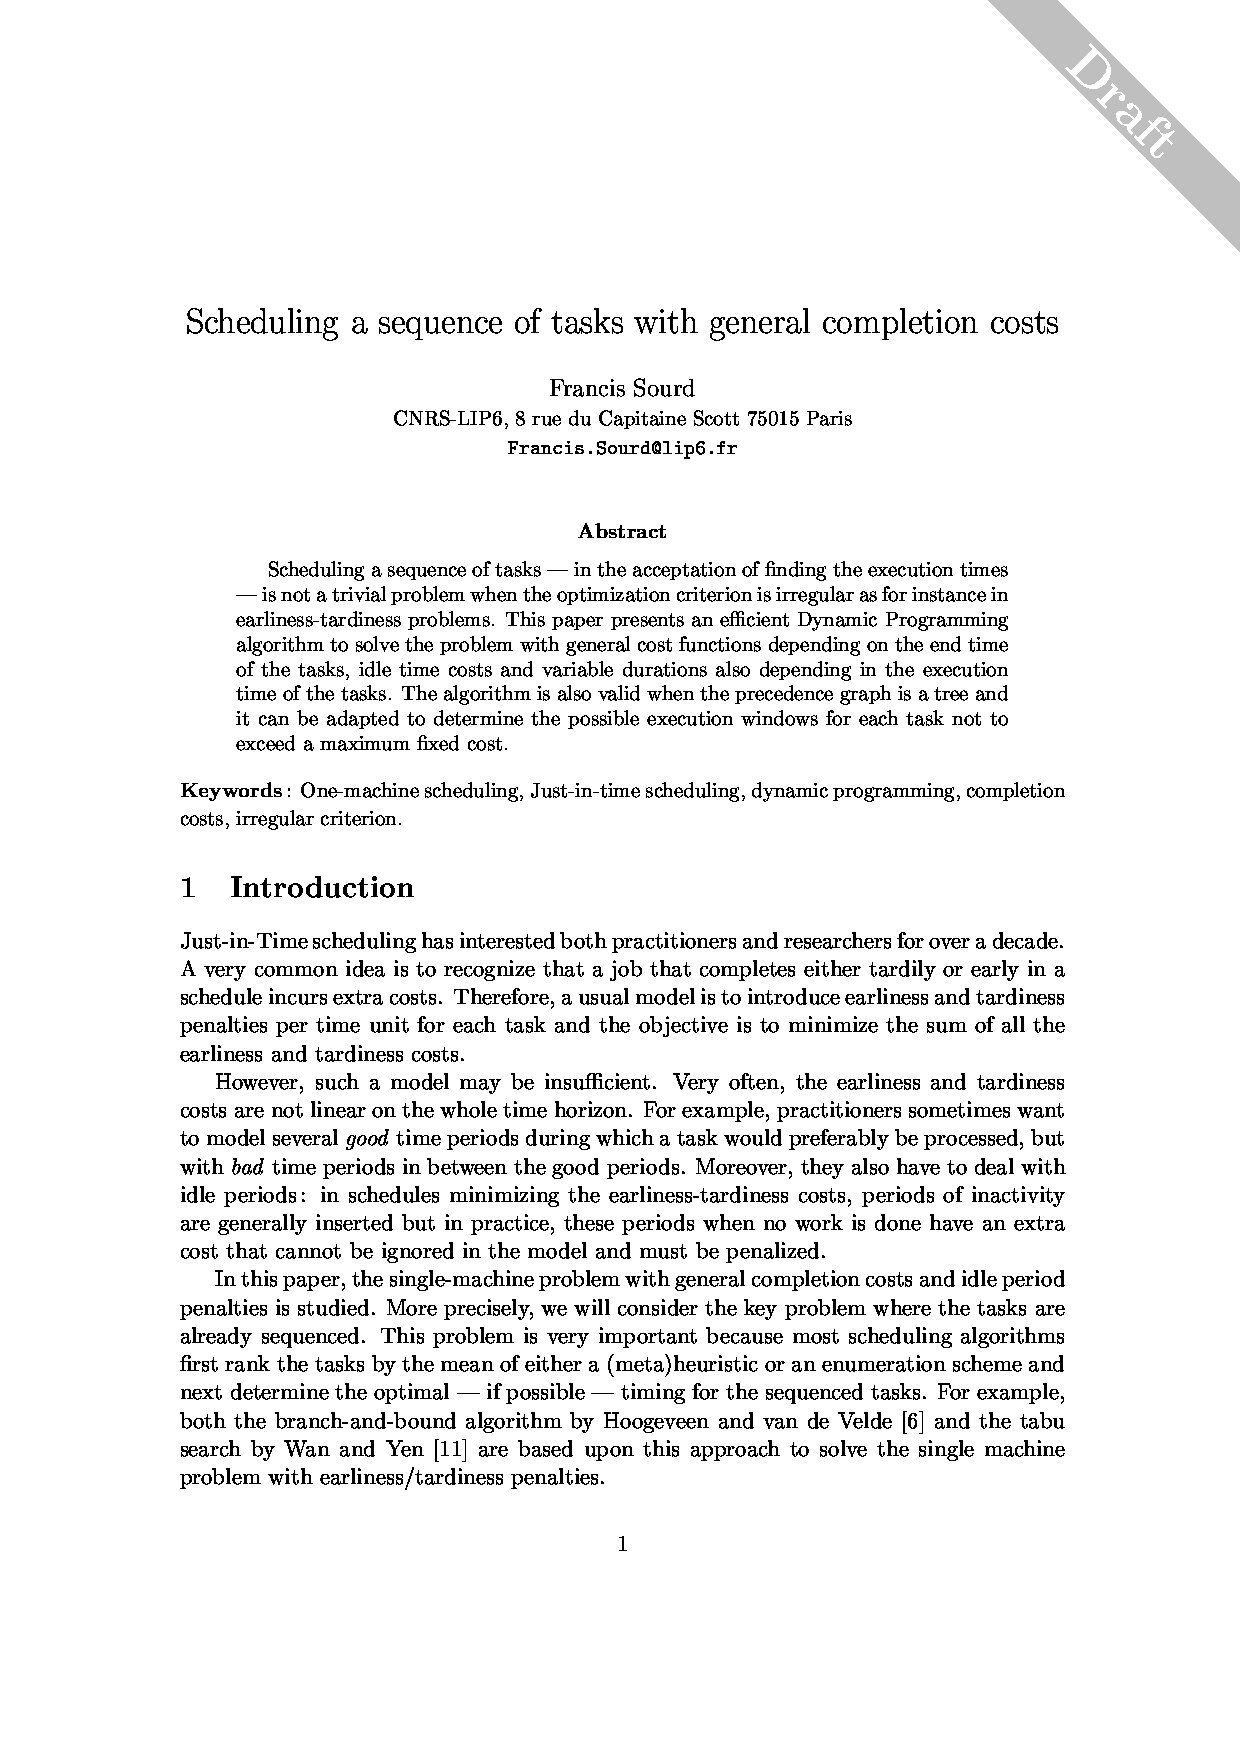
\includegraphics[width=5.5cm,keepaspectratio,clip]{sequence.pdf}
\caption{Example of sequence variables and constraints}
\label{fig:sequence}
\end{figure}

\subsection{Comparison with Existing Frameworks}
In Constraint-Based Scheduling, disjunctive or unary resources are usually considered as a special case of discrete resources of unit capacity \cite{CPMarch2008}. As such, null-duration activities do not require any capacity of the resource and are systematically ignored. The notion of optional intervals in our framework allows a clear separation between the notions of ignored interval (non-executed) and zero-duration interval. All executed intervals, even zero-duration ones, are sequenced. This is for instance useful for modeling problems like the Traveling Salesman Problem for which the visit of a city can be modeled by a zero-duration interval variable.

%Having a sequence or a set of sequence constraints on integer variables actually misses to express in a compact and efficient way constraints in-between variables in the sequence as $\first$, $\last$, or $\prev$, but even worse constraints between sequences or a sequences and some function of time.
Due to the fact that the concept of sequence is isolated and identified as a decision variable of the model, the design is very flexible and can be extended to support expressions or constraints over sequence variables such as the transition constraints presented in \cite{Bartak2007a} or constraints that enforce other temporal relation than no-overlap.  

\section{Cumul Function Expressions}

\subsection{Usage and Rationale}

In scheduling problems involving cumulative resources, the cumulated usage of the resource by the activities is usually represented by a function of time. An activity increases the cumulated resource usage function at its start time and decreases it when it releases the resource at its end time. For resources that can be produced and consumed by activities (for instance the content of an inventory or a tank), the resource level can also be described as a function of time: production activities will increase the resource level whereas consuming activities will decrease it. In these problem classes, constraints are imposed on the evolution of these functions of time, for instance a maximal capacity or a minimum safety level. \cp\ introduces the notion of a {\em cumul function expression} which is a constrained expression that represents the sum of individual contributions of intervals.\footnote{In the rest of the paper, we often drop ``expression'' from ``cumul function expression'' to increase readability.} A set of elementary cumul functions is available to describe the individual contribution of an interval variable or a fixed interval of time. These elementary functions cover the use-cases mentioned above: {\em pulse} for usage of a cumulative resource, and {\em step} for resource production/consumption. When the elementary cumul functions that define a cumul function are fixed (and thus, so are their related intervals), the cumul function itself is fixed and its value is a stepwise integer function. Several constraints are provided over cumul functions. These constraints allow restricting the possible values of the function over the complete horizon or over some fixed or variable interval.

\subsection{Formal semantics}

Let $\cal{F}^+$ denote the set of all functions from $\Z$ to $\Z^+$. A {\em
cumul function expression} $f$ is an expression whose value is a function of
$\cal{F}^+$. Let $u,v \in \Z$ and $h, h_{min}, h_{max} \in \Z^+$ and $a$ be an interval variable, we consider {\bf elementary cumul functions} illustrated in Figure \ref{fig:shapes}.

\begin{figure}[ht]
\centering
\includegraphics[width=7cm,keepaspectratio,clip]{shapes.pdf}
\caption{Elementary cumul function expressions}
\label{fig:shapes}
\end{figure}

Whenever the interval variable of an elementary cumul function is not executed, the function is the zero function. A {\bf cumul function} $f$ is an expression built as the algebraic sum of the elementary functions of Figure \ref{fig:shapes} or their negations. More formally, it is a construct of the form $f = \sum_i \epsilon_i \cdot f_i$ where $\epsilon_i \in \{-1,+1\}$ and $f_i$ is an elementary cumul function. 

The following constraints can be expressed on a cumul function $f$ to restrict its possible values:
\begin{itemize}
\item $\alwaysIn(f,u,v,h_{min},h_{max})$ means that the values of function $f$ must remain in the range $[h_{min},h_{max}]$ everywhere on the interval $[u,v)$.
\item $\alwaysIn(f,a,h_{min},h_{max})$ means that if interval $a$ is executed,
the values of function $f$ must remain in the range $[h_{min},h_{max}]$ between the start and the end of interval variable $a$.
\item $f \leq h$: function $f$ cannot take values greater than $h$. 
\item $f \geq h$: function $f$ cannot take values lower than $h$. 
\end{itemize}

An integer expression is introduced to get the total contribution of an interval variable $a$ to a cumul function $f$ at its start: $\heightAtStart(a,f,dh)$ with a default value $dh$ in case $a$ is not executed. A similar expression exists for the end point. These expressions are useful to constrain the variable height of an elementary cumul function specified as a range $[h_{min},h_{max}]$ using classical constraints on integer expressions.

\subsection{Example}

The constraints below model (1) a set of $n$ activities $\{a_i\}$ such that no more than $3$ activities in the set can overlap and (2) a chain of optional interval variables $w_j$ that represent the distinct time-windows during which at least one activity $a_i$ must execute. The constraints on interval variable status ensure that only the first intervals in the chain are executed and the two $\alwaysIn$ constraints state the synchronization relation between intervals $a_i$ and intervals $w_j$. A solution is illustrated on Figure \ref{fig:solcumul}.
\small
\begin{eqnarray*}
f_a = \sum_{i=1}^{n} \pulse(a_i,1);  && f_w = \sum_{j=1}^{n} \pulse(w_j,1); \\
&& f_a \leq 3; \\
\forall j \in [1,n-1] & &
\left \lbrace
\begin{array}{l}
  \exec(w_{j+1}) \Rightarrow \exec(w_j); \\
  \EndBeforeStart(w_j, w_{j+1});
\end{array}
\right. \\
\forall i \in [1,n]   & & 
\left \lbrace
\begin{array}{l}
  \alwaysIn(f_a,w_i,1,n); \\
  \alwaysIn(f_w,a_i,1,1);
\end{array}
\right. 
\end{eqnarray*}
\normalsize

\begin{figure}[ht]
\centering
\includegraphics[width=6.5cm,keepaspectratio,clip]{solcumul.pdf}
\caption{Covering chain}
\label{fig:solcumul}
\end{figure}

\subsection{Comparison with Existing Frameworks}

Cumul functions subsume the classical discrete cumulative resources in Constraint-Based scheduling (discrete or reusable resources and discrete reservoirs) such as the ones used in IBM ILOG Scheduler \cite{CPMarch2008} or predefined in EUROPA2 \cite{Frank2003}. In particular, minimal and maximal capacity profiles can be expressed by $\alwaysIn$ constraints on fixed intervals.

Cumul functions and their constraints are close to the {\em Resource Temporal Network} formalism proposed in \cite{Laborie2003}. Elementary cumul functions represent {\em relative changes} whereas $\alwaysIn$ constraints cover both {\em lower-than} and {\em greater-than} conditions. It is possible to model {\em absolute change} -- setting the current value of the function to $v$ -- by a combination of a $\stepAtStart(a, 0, \infty)$ with variable height and a constraint $\alwaysIn(a,v,v)$ stating that the target value is $v$. This can be used for instance to model an activity that empties a tank ($v=0$). This bridge between the two formalisms shows the additional expressive power of the $\alwaysIn$ constraint: as this constraint can hold on variable intervals, it introduces the AI Planning notion of condition in the constrained-based scheduling world. Note that this type of $\alwaysIn$ constraint is easy to express in our formalism because the notion of cumul function is isolated as an expression. It would be much harder to express in a formalism based solely on integer variables.

\section{State Function Variables}

\subsection{Usage and Rationale}

In the same way as the value of an integer variable may represent an ordinal integer, functions over ordinal integers are useful in scheduling to describe the time evolution of a state variable. Typical examples are the time evolution of an oven's temperature, of the type of raw material present in a tank or of the  tool installed on a machine. To that end, we introduce the notion of a {\em state function variable} and a set of constraints similar to the $\alwaysIn$ constraints on cumul functions to constrain the values of the state function. 

A state function is a set of non-overlapping intervals over which the function maintains a constant non-negative integer state. In between those intervals, the state of the function is not defined. For instance for an oven with 3 possible temperature levels identified by indices $0$, $1$ and $2$ we could have the following time evolution (see also Figure \ref{fig:state}):

\vspace*{2mm}
\begin{tabular}{lll}
$[\Start=0$,   & $\End=100)$: & $\state=0$, \\
$[\Start=140$, & $\End=300)$: & $\state=1$,\\
$[\Start=320$, & $\End=500)$: & $\state=2$,\\
$[\Start=540$, & $\End=600)$: & $\state=2, \cdots$ \\
\end{tabular}\\

\subsection{Formal Semantics}

\subsubsection{State Function Variable.}


A {\bf state function variable} $f$ is a variable whose value is a set of non-overlapping intervals, each interval $[s_i,e_i)$ (with $s_i < e_i$) is associated with a non-negative integer value $v_i$ that represents the state of the function over the interval. Let  $\underline{f}$ be a fixed state function, we will denote $\underline{f}=(\ [s_i,e_i):v_i\ )_{i \in [1,n]}$. We denote $D(\underline{f})= \cup_{i \in [1,n]}[s_i,e_i)$ the definition domain of $\underline{f}$, that is, the set of points where the state function is associated a state. For a fixed state function $\underline{f}$ and a point $t \in D(\underline{f})$, we will denote $[s(\underline{f},t),e(\underline{f},t))$ the unique interval of the function that contains $t$ and $\underline{f}(t)$ the value of this interval. For instance, in the oven example we would have $\underline{f}(200)=1$, $s(\underline{f},200)=140$ and $e(f,200)=300$.

A state function can be endowed with a {\bf transition distance}. The transition distance defines the minimal distance that must separate two consecutive states in the state function. More formally, if $M[v,v']$ is a transition distance matrix between state $v$ and state $v'$, we have: $\forall i \in [1,n-1], \ e_i + M[v_i,v_{i+1}] \leq s_{i+1}$.

\begin{figure}[ht]
\centering
\includegraphics[width=8cm,keepaspectratio,clip]{state.pdf}
\caption{State function}
\label{fig:state}
\end{figure}

\subsubsection{Constraints on State Functions}

If $f$ is a state function of definition domain $D(f)$, $a$ an interval variable, $v$, $v_{min} \leq v_{max}$ non-negative integers and $\algn_s$, $\algn_e$ two boolean values:
\begin{itemize}
\item The constraint $\alwaysConstant(f,a,\algn_s,\algn_e)$ specifies that whenever $a$ is executed, the function takes a constant value between the start and the end of $a$. Boolean parameters $algn$ allow specifying whether or not interval variable $a$ is synchronized with the start (resp. end) of the state function interval:
\begin{enumerate}
  \item[(a)] $[s(\underline{a}),e(\underline{a})) \subset [s(\underline{f},s(\underline{a})), e(\underline{f},s(\underline{a})))$ 
  \item[(b)] $\algn_s \Rightarrow s(\underline{a})=s(\underline{f},s(\underline{a}))$
  \item[(c)] $\algn_e \Rightarrow e(\underline{a})=e(\underline{f},e(\underline{a}))$ 
  \item[(d)] $\exists v \in \Z^+, \forall t \in  [s(\underline{a}),e(\underline{a})), \underline{f}(t)=v$
  \end{enumerate}

\item The constraint $\alwaysEqual(f,a,v,\algn_s,\algn_e)$ specifies that whenever $a$ is executed the state function takes a constant value $v$ over interval $a$:
\begin{enumerate}
  \item[(a)] $\alwaysConstant(\underline{f},\underline{a},\algn_s,\algn_e)$
  \item[(b)] $v = \underline{f}(s(\underline{a}))$
  \end{enumerate}
\item The constraint $\alwaysNoState(f,a)$ specifies that if $a$ is executed, it must not intersect the definition domain of the function, $[s(\underline{a}),e(\underline{a})) \cap D(\underline{f})=\emptyset$.
\item The constraint $\alwaysIn(f,a,v_{min},v_{max})$ where $0 \leq v_{min} \leq v_{max}$ specifies that whenever $a$ is executed, $\forall t \in [s(\underline{a}),e(\underline{a})) \cap D(\underline{f}), \ \underline{f}(t) \in [v_{min},v_{max}]$.
\end{itemize}

Those constraints are also available on a fixed interval $[\Start,\End)$ as well as on an interval variable.

On Figure \ref{fig:state}, interval variables $b_0:[0, 100)$ and $b_1:[140, 300)$ are start and end aligned and thus, define two segments of the state function (of respective state $0$ and $1$). A transition distance $40$ applies in between those states. Interval variable $b_{21}$ is start aligned and interval $b_{22}$ is end aligned both of state $2$. As the transition distance $2 \rightarrow 2$ is greater than $s(b_{22}) - e(b_{21})$, the state function is aligned on $[s(b_{21}),e(b_{22})= [320,500)$. Interval variable $c$ is constrained to be scheduled in an interval where the function is not defined. Finally, interval variables $a_1$, $a_2$ and $a_3$ require a particular state of the function, possibly with some alignment constraint as for $a_1$.

\subsection{Example}

The problem is to cook $n$ items with an oven, each item $i \in [1,n]$ being cooked at a specific temperature $v_i$ and for a specific range of duration. Items that are compatible both in temperature and in duration can be batched together and cooked simultaneously. Between two batches, a delay must elapse for cooling, emptying, loading, and heating the oven. For energy saving reasons the maximum reachable temperature is limited by $v_{sup}$ over some time periods. The oven can be modeled as state function with a transition distance $M$. Each item is an interval variable $a_i$, possibly optional if the problem is over-constrained so that not all items can be cooked, and states an $\alwaysEqual$ constraint with start and end alignment. Each energy saving window is a fixed interval $[s_j,e_j)_{j \in [1,m]}$ that states an $\alwaysIn$ constraint: 

\vspace*{-2mm}
\small
\[
\begin{array} {l}
\forall i \in [1,n], \alwaysEqual(oven, a_i, v_i, true, true); \\
\forall j \in [1,m], \alwaysIn(oven, s_j, e_j, 0, v_{sup});\\ 
\end{array} \]
\normalsize

\subsection{Comparison with Existing Frameworks}

State function variables and related constraints subsume the state resources and type timetable constraints on discrete resources \cite{CPMarch2008} available in some Constraint-Based Scheduling systems. In practice, alignments, no state and transition distance allow defining a sequence of states in the schedule without knowing {\em a priori} the sequenced intervals and their types. As a consequence, coupled with cumul functions, state functions allow elegant models that permits the generic expression of different types of temporal incompatibilities and synchronization between activities of a resource.

\section{Constraint Propagation and Search}

\cp\ implements a robust search algorithm to support the formalism described in this paper. This search was tested on an extensive library of models. It is based on the Self-Adapting Large Neighborhood Search described in \cite{Laborie2007} that consists of an improvement method that iteratively {\em unfreezes} and {\em re-optimizes} a selected fragment of the current solution. 

Unfreezing a fragment relies on the notion of Partial Order Schedule \cite{Policella2004}. This notion has been generalized to the modeling elements presented in this paper (no-overlap constraint, cumul function expressions and state variables). 

The re-optimization of a partially unfrozen solution relies on a tree search using constraint propagation techniques. Classical constraint propagation algorithms have been extended to be able to handle optional interval variables and additional constraints. These algorithms include: time-tabling, precedence graphs or disjunctive constraint \cite{Baptiste2001} and edge-finding variants \cite{Vilim2007PhD}. For instance, for cumul functions, time-tabling algorithm has been extended to handle $\alwaysIn$ constraints on interval variables. For state functions, the time-tabling and disjunctive algorithms have been extended to handle the alignment specifications and the various types of incompatibilities between the $\alwaysIn$, $\alwaysConstant$, $\alwaysEqual$ and $\alwaysNoState$ constraints.

By default, light propagation algorithms with an average linear complexity are used. A set of inference level parameters is available to the user to perform additional filtering as summarized on Table \ref{tab:ConstraintPropagationAlgorithms}.

\begin{table}[h]
\small
\begin{tabular}{|l|l|l|} \hline
{\bf Model element} & {\bf Inference level} & {\bf Filtering algorithms} \\ \hline 
Sequence          & {\bf Basic}   & Light precedence graph \\ 
variable          & $\geq$ Medium & Precedence graph \\ \hline 
No-overlap        & {\bf Basic}   & Timetable \\
constraint        & Medium        & + Disjunctive \\
                  & Extended      & + EF variants \\ \hline
Cumul function    & {\bf Basic}   & Timetable \\
expression        & Medium        & + Disjunctive \\
                  & Extended      & + EF variants \\ \hline
State function    & {\bf Basic}   & Timetable \\
variable          & $\geq$ Medium & + Disjunctive \\ \hline
\end{tabular}
\caption{Constraint propagation algorithms}
\label{tab:ConstraintPropagationAlgorithms}
\end{table}
\normalsize

\section{Conclusion}

The algebraic model presented in this paper has been implemented in IBM ILOG \cp\ and is available in C++, Java, C\# as well as in the OPL Optimization Programming Language \cite{Laborie2008}. In complement of the notion of {\em optional interval variable} that considerably simplifies the modelling of complex scheduling structures (optional activities, alternative modes or recipes), a set of global variables and expressions has been introduced for each aspect of a scheduling problem: {\em sequence variables} for interval sequencing, {\em cumul function expressions} for cumulative reasoning and {\em state function variables} for representing the time evolution of a state variable. A powerful set of constraints on these variables and expressions is provided. As all these constraints handle the optional status of interval variables, they can be posted even on optional or alternative parts of the schedule to effectively prune part of the search space.

The clear separation between (1) the structure of scheduling problems captured with composition constraints on optional interval variables such as {\em span} and {\em alternative} and (2) the resource constraints expressed as mathematical concepts such as sequences or functions results in very simple, elegant and concise models. For instance, the model for the classical Multi-Mode Resource-Constrained Project Scheduling Problem with both renewable and non-renewable resources is less than 50 lines long in OPL including data manipulation. 

The automatic search algorithm has shown to be robust and efficient for solving a large panel of models as shown in \cite{Laborie2007} in a preliminary study. 

%global variables and interval variables state the timely local conditions to enforce. Last, as well as for Interval Variables, Integer Expressions on the timely local content of the global variables links the scheduling model to the integer model part. 

%In fact, this  language is both an extension of Constraint Based Scheduling implementations and of classical Integer Constraint Programming languages: the definition of Scheduling oriented decision and global variables avoid  global constraints that are hard to locally manipulate and  unfreeze the too strong semantic of the notion of activity and resources. From a model point of view, we both keep, and even augment, the design capability of Constraint Based Scheduling and the versatility of Integer Constraint Programming. From a search point of view, we lean on strong structural properties both to choose the suited propagation algorithms, the solution buildings, and heuristics for optimization.

%For extending model performances for complex problem, we want investigate more constraints involving sequence variables as well as numerical expressions involving functions. 

\noindent

\bibliography{biblio}
\bibliographystyle{aaai}
\end{document}
